\usetikzlibrary{calc}
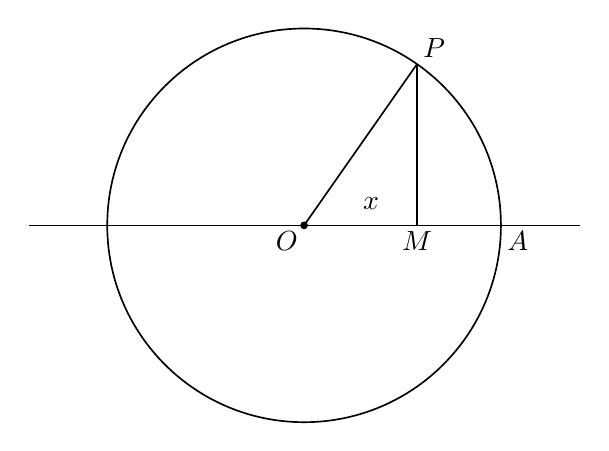
\begin{tikzpicture}[x=1cm,y=1cm,line width=.6pt,font=\normalsize]
\coordinate (O) at (0,0);
\coordinate (A) at (2.5,0);
\coordinate (P) at (1.433941,2.04788);
\coordinate (M) at (1.433941,0);
\coordinate (L) at (-3.5,0);
\coordinate (Rr) at (3.5,0);
\draw (O) circle[radius=2.5cm];
\draw (L)--(Rr);
\draw (O)--(P);
\draw (P)--(M);
\node at (0.85,0.28) {$x$};
\node[below left=2pt,inner sep=0pt] at (O) {$O$};
\node[below right=2pt,inner sep=0pt] at (A) {$A$};
\node[above right=2pt,inner sep=0pt] at (P) {$P$};
\node[below=2pt,inner sep=0pt] at (M) {$M$};

% Explicit named circle-center points, painted after all region fills.
\fill (O) circle[radius=1.4pt];
\end{tikzpicture}
